\section{Consensus}

\begin{frame}
    \frametitle{What is Consensus?}
    \begin{itemize}
        \item Agreememt on shared state(single system image)
        \item Recovers from server failure autonomously
            \begin{itemize}
                \item Minority of servers fail: no problem
                \item Majority fail: lose availability, retain consistency
            \end{itemize}
        \begin{figure}
            \centering
            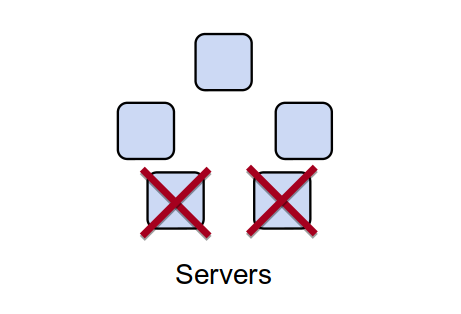
\includegraphics[scale=0.3]{concensus.png}
        \end{figure}
        \item Key to building consistent storage systems.
    \end{itemize}
\end{frame}

\begin{frame}
    \frametitle{To eliminate single point of failure: Replication}
    \begin{itemize}
        \item Network partition or server down
        \item Consensus
            \begin{itemize}
                \item Allows collection of machines to work as coherent group
                \item Continuous service, even if some machines fail
            \end{itemize}
        \item A concensus algorithm(built-in or library)
            \begin{itemize}
                \item Paxos(1990) has dominated discussion for 25 years, hard for engineer.
                \item Raft(2013) is easier to understand.
                \item \ldots
            \end{itemize}
        \item A concensus service
            \begin{itemize}
                \item Google Chubby
                \item Apache ZooKeeper
                \item \ldots
            \end{itemize}
    \end{itemize}
\end{frame}

\begin{frame}
    \frametitle{Replicated State Machine(RSM)}
    \begin{figure}
       \centering
        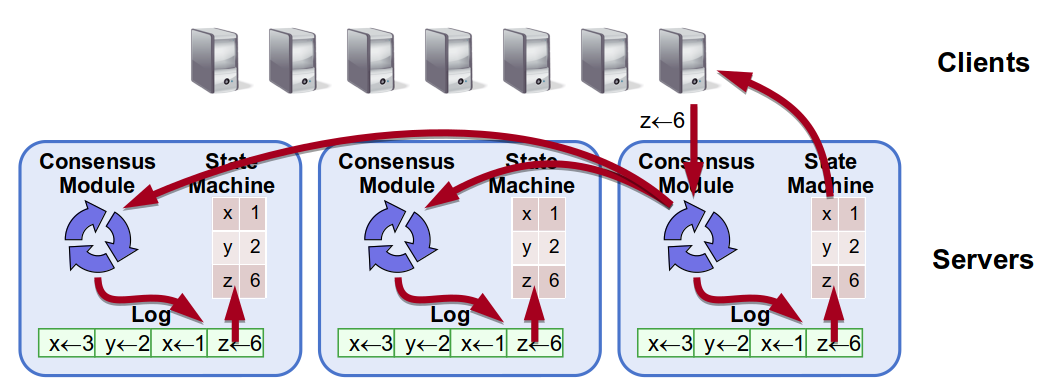
\includegraphics[scale=0.3]{rsm.png}
    \end{figure}

    \begin{itemize}
        \item Replicated log => \alert{All servers execute same commands in same order}.
        \item Consensus module ensures proper log replication.
        \item System makes progress as long as any majority of servers are up.
        \item Failure model: fail-stop(not Byzantine), delayed/lost messages.
    \end{itemize}
\end{frame}

%\subsection{Raft}

\begin{frame}
    \frametitle{Raft Overview}
    \begin{itemize}
        \item Leader election
            \begin{itemize}
                \item Select one of servers to act as cluster leader
                \item Detect crashes, choose new leader
            \end{itemize}
        \item Log replication
            \begin{itemize}
                \item Leader takes commands from clients, appends them to its log.
                \item Leader replicates its log to other servers(overwriting inconsistencies)
            \end{itemize}
        \item Safety: Only a server with an up-to-date log can become leader.
    \end{itemize}
\end{frame}

\begin{frame}
    \centering
    \href{http://thesecretlivesofdata.com/raft/}{Raft Visualization}
\end{frame}

\begin{frame}
    \frametitle{Core Raft Overview}
    \begin{itemize}
        \item Leader election
            \begin{itemize}
                \item Heartbeats and timeouts to detect crashes
                \item Randomized timeouts to avoid split votes
                \item Majority voting to guarantee at most one leader per term
            \end{itemize}
        \item Log replication
            \begin{itemize}
                \item Leader takes commands from clients, appends them to its log.
                \item Leader replicates its log to other servers(overwriting inconsistencies)
            \end{itemize}
        \item Safety
            \begin{itemize}
                \item Only elect leaders with all committed entries in their logs.
                \item New leader defers committing entries from prior terms.
            \end{itemize}
    \end{itemize}
\end{frame}

\begin{frame}
    \frametitle{Server States}
    \begin{itemize}
        \item \textbf{At any given time, each server is either:}
            \begin{itemize}
                \item \alert{Leader}: handles all client interactions, log replication
                \item \alert{Followers}: completely passive(issue no RPCs, responds to incoming RPCs)
                \item \alert{Candidate}: used to elect a new leader
            \end{itemize}
        \item \textbf{Normal operation: 1 leader, N-1 followers}
    \end{itemize}
    \begin{figure}
        \centering
        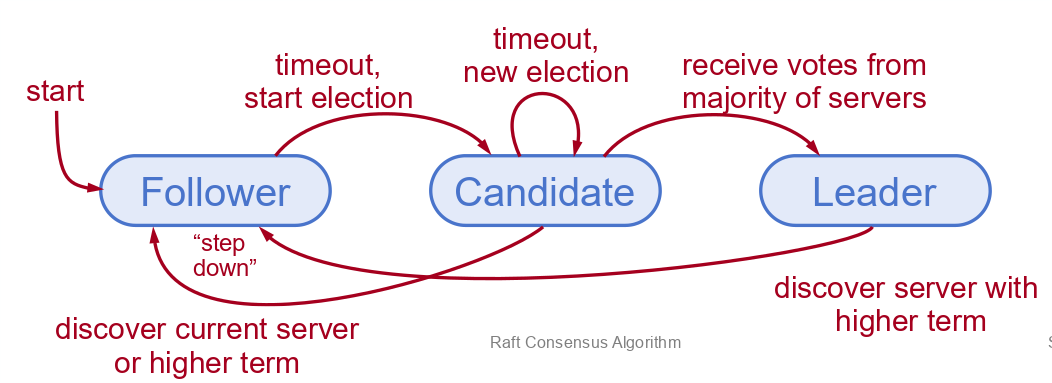
\includegraphics[scale=0.3]{raft-servers.png}
    \end{figure}
\end{frame}

\begin{frame}
    \frametitle{Terms}
    \begin{figure}
        \centering
        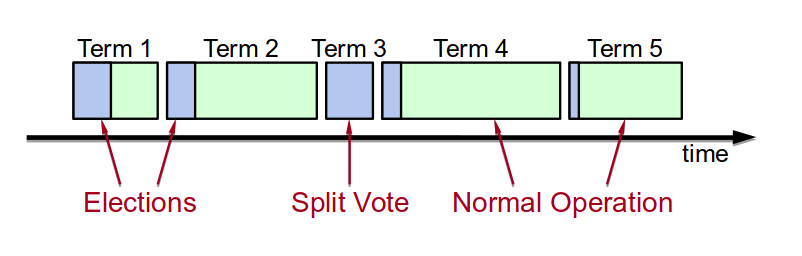
\includegraphics[scale=0.3]{raft-terms.png}
    \end{figure}
    \begin{itemize}
        \item \textbf{Time divided into terms:}
            \begin{itemize}
                \item Election
                \item Normal operation under a single leader
            \end{itemize}
        \item \textbf{At most 1 leader per term}
        \item \textbf{Some terms have no leader(failed election)}
        \item \textbf{Each server maintains \alert{current term} value}
        \item \textbf{\alert{Key role of terms: identify obsolete information}}
    \end{itemize}
\end{frame}

\begin{frame}
    \frametitle{Raft Remote Procedure Calls(RPCs)}
    \begin{itemize}
        \item \textbf{Raft servers using RPCs to communicate}
            \begin{itemize}
                \item RPC is a key piece of distribute system machinery
                \item RPC ideally make net communication look just like function call
            \end{itemize}
        \begin{figure}
            \centering
            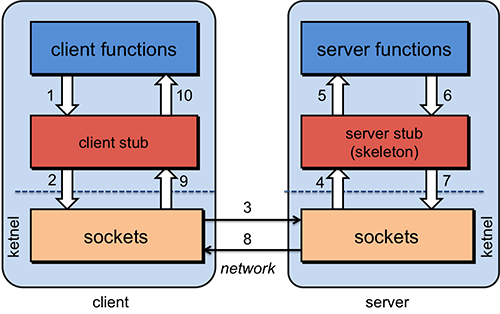
\includegraphics[scale=0.5]{rpc-flow.png}
        \end{figure}
        \item \textbf{RequestVote RPC}
            \begin{itemize}
                \item Invoked by candidate to gather votes
            \end{itemize}
        \item \textbf{AppendEntries RPC}
            \begin{itemize}
                \item Invoked by leader to replicate log entries
                \item Also used as heartbeats
            \end{itemize}
    \end{itemize}
\end{frame}

\begin{frame}
    \frametitle{RequestVote RPC}
    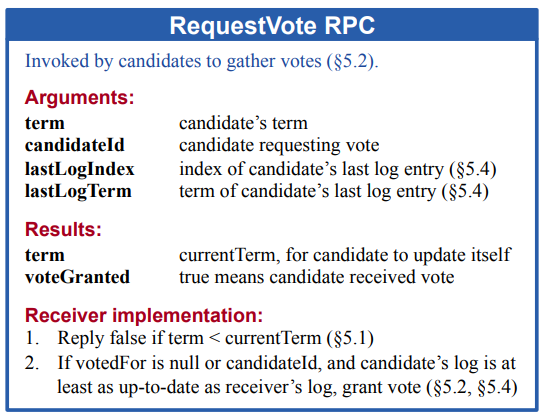
\includegraphics[scale=0.3]{raft-requestvote.png}
\end{frame}

\begin{frame}
    \frametitle{AppendEntries RPC}
    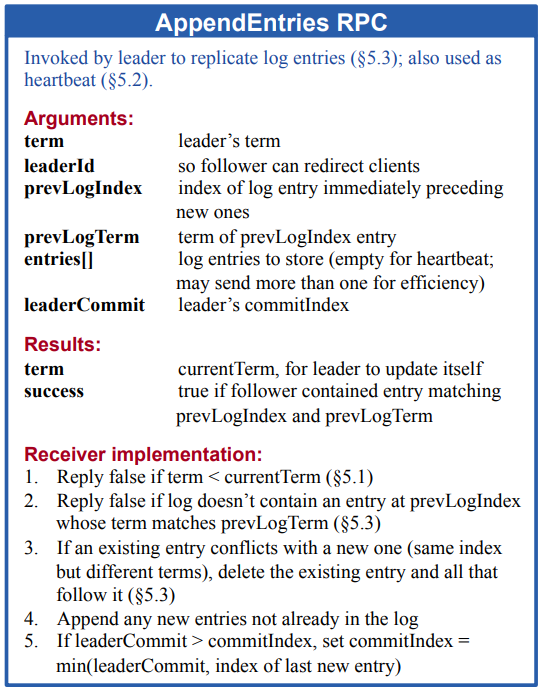
\includegraphics[scale=0.3]{raft-appendentries.png}
\end{frame}

\begin{frame}
    \frametitle{Heartbeats and Timeouts}
    \begin{itemize}
        \item \textbf{Servers start up as followers}
        \item \textbf{Followers expect to receive RPCs from leaders or candidates}
        \item \textbf{Leaders must send \alert{heartbeats}(empty AppendEntries RPCs) to maintains authority}
        \item \textbf{If \alert{election Timeout} elapses with no RPCs:}
            \begin{itemize}
                \item Follower assumes leader has crashed
                \item Follower starts new election
                \item Timeouts typically 100-500 ms
            \end{itemize}
    \end{itemize}
\end{frame}

\begin{frame}
    \frametitle{Election Basics}
    \begin{itemize}
        \item \textbf{Increment current term}
        \item \textbf{Change to Candidate state}
    \item \textbf{Vote for self}
    \item \textbf{Send RequestVote RPCs to all other servers, retry until either:}
            \begin{itemize}
                \item Receive votes from majority of servers:
                    \begin{itemize}
                        \item Become leader
                        \item Send AppendEntries heartbeats to all other servers
                    \end{itemize}
                \item Receive RPC from valid leader:
                    \begin{itemize}
                        \item Return to follower state
                    \end{itemize}
                \item No-one wins election(election timeout elapses):
                    \begin{itemize}
                        \item Increment term, start new election
                    \end{itemize}
            \end{itemize}
    \end{itemize}
\end{frame}

\begin{frame}
    \frametitle{Elections, cont'd}
    \begin{itemize}
        \item \textbf{\alert{Safety}: allow at most one winner per term}
            \begin{itemize}
                \item Each server gives out only one vote per term(persist on disk)
                \item Two different candidates can't accumulate majorities in same term
            \end{itemize}
        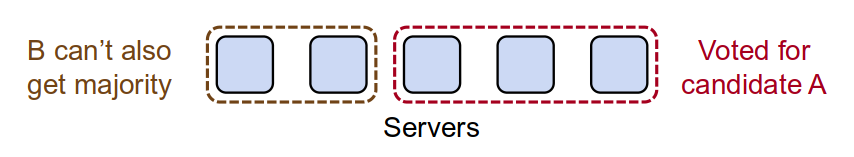
\includegraphics[scale=0.3]{raft-safety.png}
        \item \textbf{\alert{Liveness}: some candidate must eventually win}
            \begin{itemize}
                \item Choose election timeouts randomly in [T, 2T]
                \item One sever usually times out and wins election before others wake up
                \item Works well if T $\gg$ broadcast time
            \end{itemize}
    \end{itemize}
\end{frame}

\begin{frame}
    \frametitle{Log Structure}
    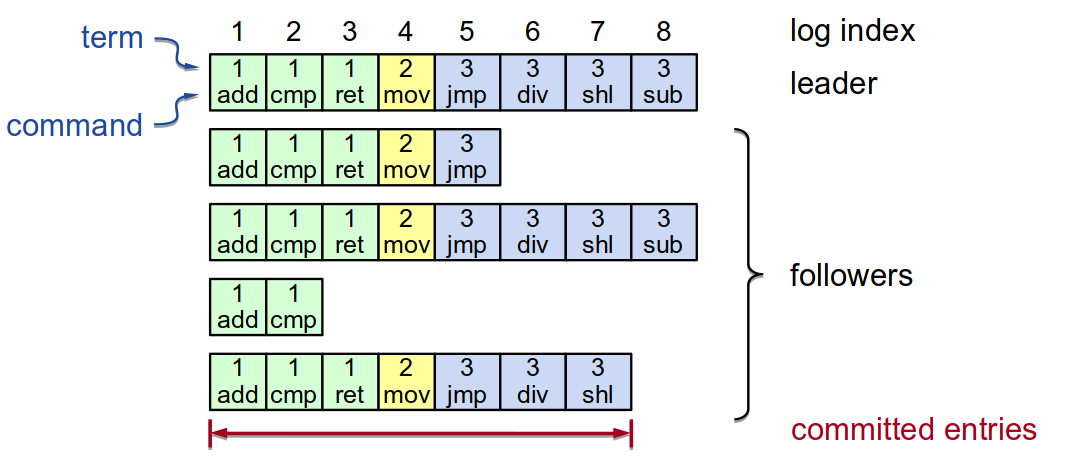
\includegraphics[scale=0.3]{raft-log.png}
    \begin{itemize}
        \item Log entry = index, term, command
        \item Log stored on stable storage(disk); survives crashes
        \item Entry \alert{committed} if known to be stored on majority of servers
            \begin{itemize}
                \item Durable, will eventually be executed by state machines
            \end{itemize}
    \end{itemize}
\end{frame}

\begin{frame}
    \frametitle{Normal Operation}
    \begin{itemize}
        \item \textbf{Client sends command to leader}
        \item \textbf{leader appends command to its log}
        \item \textbf{Leader sends AppendEntries RPCs to followers}
        \item \textbf{Once new entry committed:}
            \begin{itemize}
                \item Leader passes command to its state machine, returns result to client
                \item Leader notifies followers of committed entries in subsequent AppendEntries RPCs
                \item Followers pass committed commands to their state machines
            \end{itemize}
        \item \textbf{Crashed/slow followers?}
            \begin{itemize}
                \item Leader retries RPCs until they succeed
            \end{itemize}
        \item \textbf{Performance is optimal in common case:}
            \begin{itemize}
                \item One successful RPC to any majority of servers
            \end{itemize}
    \end{itemize}
\end{frame}

\begin{frame}
    \frametitle{Log Consistency}
    \textbf{High level of conherency between logs:}
    \begin{itemize}
        \item If log entries on different servers have same index and term:
            \begin{itemize}
                \item They store the same command
                \item The logs are identitcal in all preceding entries
            \end{itemize}
        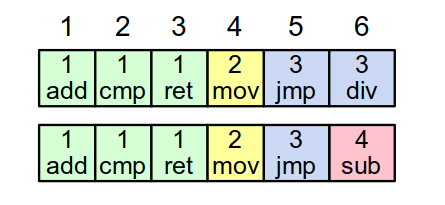
\includegraphics[scale=0.3]{raft-log2.png}
        \item If a given entry is committed, all preceding entries are also committed
    \end{itemize}
\end{frame}

\begin{frame}
    \frametitle{AppendEntries Consistency Check}
    \begin{itemize}
        \item Each AppendEntries RPC contains index, term of entry preceding new ones
        \item Follower must contain matching entry; otherwise it rejects request
        \item Implements an \alert{induction step}, ensures coherency
    \end{itemize}
    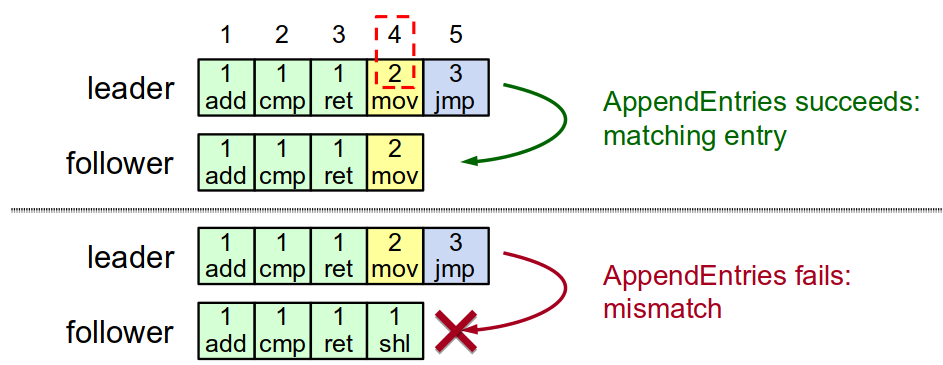
\includegraphics[scale=0.3]{raft-consistency.png}
\end{frame}

\begin{frame}
    \frametitle{Leader Changes}
    \begin{itemize}
        \item At begining of new leader's term:
            \begin{itemize}
                \item Old leader may have left entries partially replicated
                \item No special steps by new leader: just start normal operation
                \item Leader's log is \alert{the truth}
                \item Will eventually make follower's logs identical to leader's
                \item Multiple crashes can leave many extraneous log entries:
            \end{itemize}
    \end{itemize}
    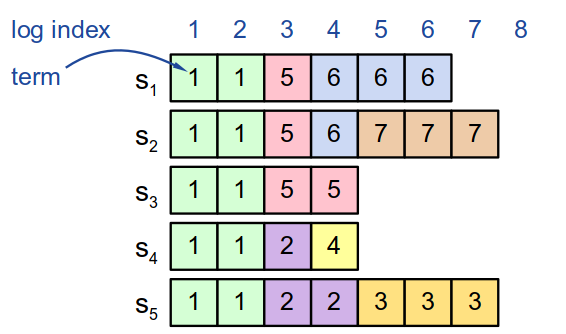
\includegraphics[scale=0.3]{raft-leader-changes.png}
\end{frame}

\begin{frame}
    \frametitle{Log Inconsistencies}
    \textbf{Leader changes can result in log inconsistencies:}
    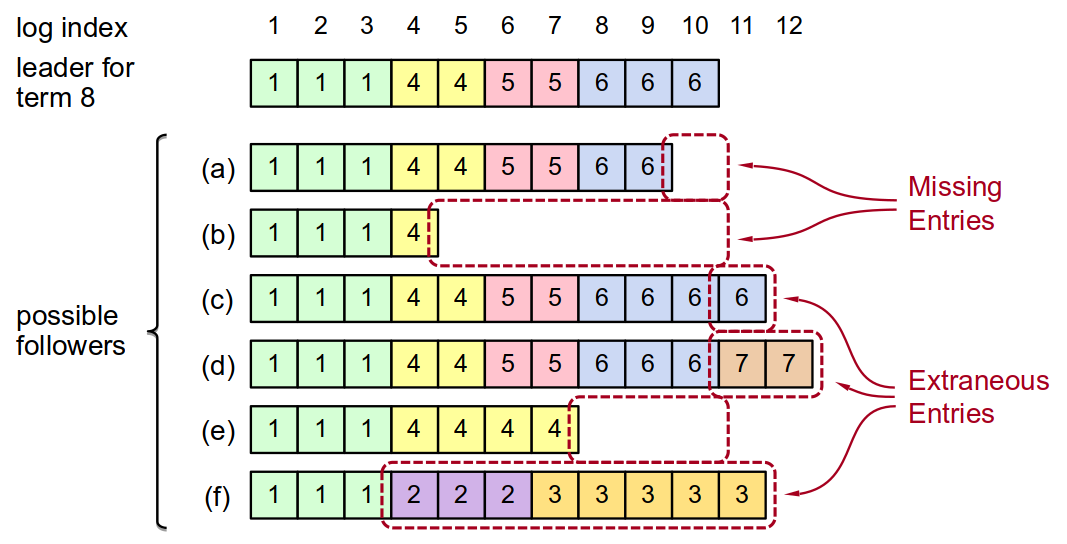
\includegraphics[scale=0.3]{raft-log-inconsistency.png}
\end{frame}

\begin{frame}
    \frametitle{Repairing Follower Logs}
    \begin{itemize}
        \item \textbf{New leader must make follower logs consistent with its own}
            \begin{itemize}
                \item Delelte extraneous entries
                \item Fill in missing entries
            \end{itemize}
        \item \textbf{Leader keeps nextIndex for each follower:}
            \begin{itemize}
                \item Index of next log entry to send to that follower
                \item Initialized to (1 + leader's last index)
            \end{itemize}
        \item \textbf{When AppendEntries Consistency Check fails, decrement nextIndex and try again:}
    \end{itemize}
    \centering
    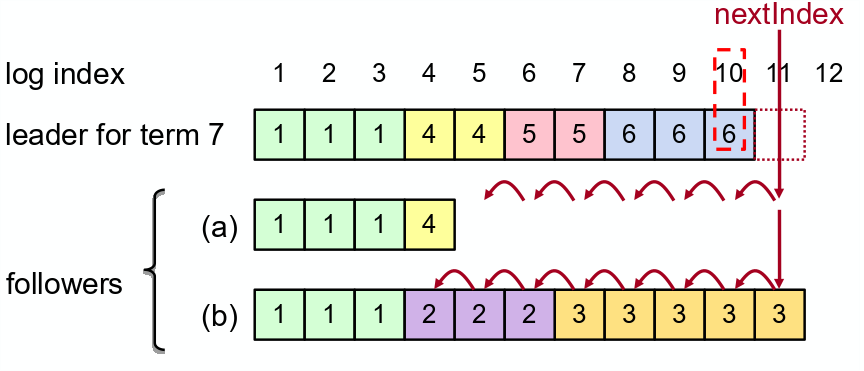
\includegraphics[scale=0.3]{raft-repairing-follower-logs.png}
\end{frame}

\begin{frame}
    \frametitle{Repairing Logs, cont'd}
    \begin{itemize}
        \item \textbf{When follower overwrites inconsistent entry, it deletes all subsequent entries:}
    \end{itemize}
    \centering
    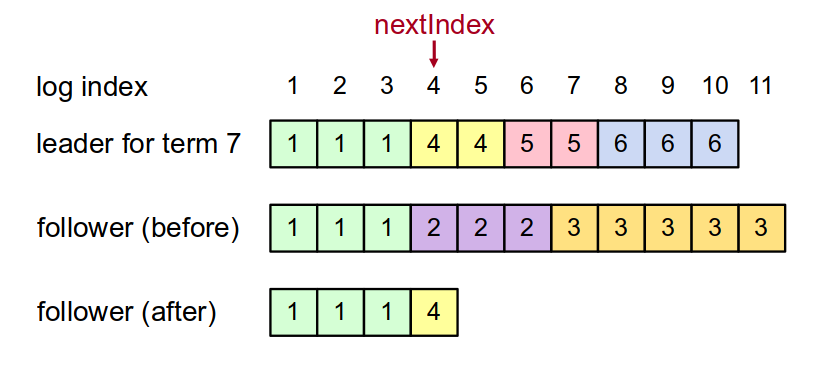
\includegraphics[scale=0.3]{raft-repariring-follower-logs2.png}
\end{frame}

\begin{frame}
    \begin{block}{Safety Requirement}
        Once a log entry has been applied to a state machine, no other state machine must apply a different value for that log entry
    \end{block}
    \begin{itemize}
        \item \textbf{Raft safety property:}
            \begin{itemize}
                \item If a leader has decided that a log entry is committed, that entry will be present in the logs of all future leaders.
            \end{itemize}
        \item \textbf{This guarantees the safety requirement}
            \begin{itemize}
                \item Leaders never overwrite entries in their logs
                \item Only entries in the leader's log can be committed
                \item Entries must be committed before applying to state machine
            \end{itemize}
    \end{itemize}
\end{frame}

\begin{frame}
    \frametitle{Picking the Best Leader}
    \begin{itemize}
        \item \textbf{Can't tell which entries are committed!}
        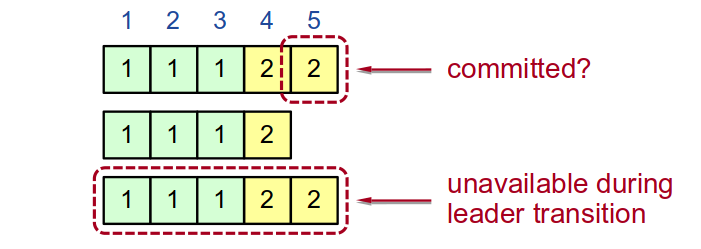
\includegraphics[scale=0.3]{raft-picking-leader.png}
        \item \textbf{During elections, choose candidate with log most likely to contain all committed entries}
            \begin{itemize}
                \item Candidates include log info in RequestVote RPCs: \\
                    (index \& term of last log entry)
                \item Voting server V denies vote if its log is 'more complete': \\
                    {\color{blue}{$(lastTerm_V > lastTerm_C) \|$}}  \\
                    {\color{blue}{$(lastTerm_V == lastTerm_C) \&\& (lastIndex_V > lastIndex_C)$}}
                \item Leader will have 'most complete' log among electing majority
            \end{itemize}
    \end{itemize}
\end{frame}

\begin{frame}
    \frametitle{Committing Entry from Current Term}
    \begin{itemize}
        \item \textbf{Case 1/2: Leader decides entry in current term is committed}
        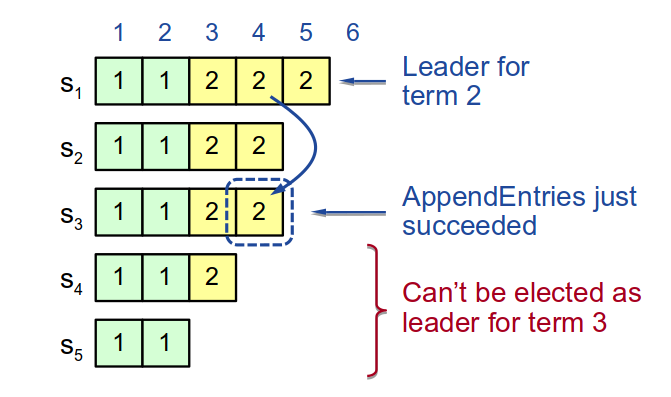
\includegraphics[scale=0.3]{raft-commit-entry.png}
        \item \textbf{Safe: leader for term 3 must contain entry 4}
    \end{itemize}
\end{frame}

\begin{frame}
    \frametitle{Committing Entry from Earlier Term}
    \begin{itemize}
        \item \textbf{Case 2/2: Leader is trying to finish committing entry from an earlier term}

        \begin{figure}
            \centering
            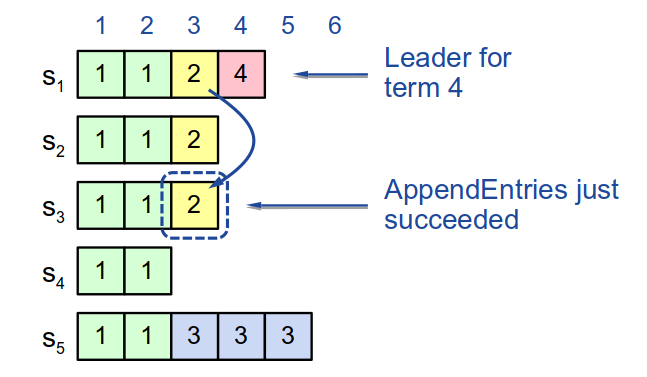
\includegraphics[scale=0.3]{raft-commite-entry2.png}
        \end{figure}

        \item \textbf{Entry 3 not safely committed:}
            \begin{itemize}
                \item $S_5$ can be elected as leader for term 5
                \item If elected, it will overwrite entry 3 on $S_1$, $S_2$, and $S_3$!
            \end{itemize}
    \end{itemize}
\end{frame}

\begin{frame}
    \frametitle{New Commitment Rules}
    \begin{minipage}{.55\textwidth}
        \begin{itemize}
            \item \textbf{For a leader to decide an entry is committed:}
                \begin{itemize}
                    \item Must be stored on a majority of servers
                    \item At least one new entry from leader's term must also be stored on majority of servers
                \end{itemize}
            \item \textbf{Once entry 4 committed:}
                \begin{itemize}
                    \item $S_5$ cannot be elected leader for term 5
                    \item Entries 3 and 4 both safe
                \end{itemize}
        \end{itemize}
    \end{minipage}
    \begin{minipage}{.4\textwidth}
        \begin{figure}[hp]
            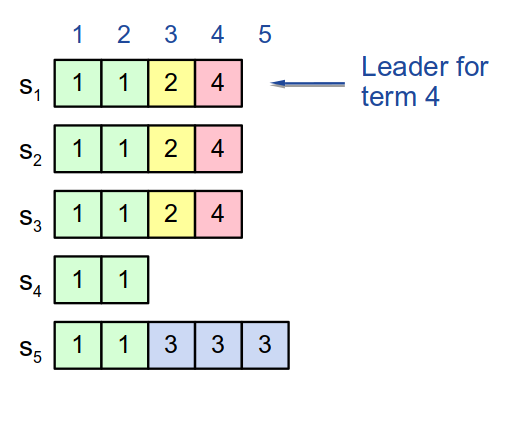
\includegraphics[scale=0.3]{raft-commit-rule.png}
        \end{figure}
    \end{minipage}
    \centering
    \textbf{Combination of election rules and Commitment rules makes Raft Safe}
\end{frame}

\begin{frame}
    \frametitle{Neutralizing Old Leaders}
    \begin{itemize}
        \item \textbf{Deposed leader may not be dead:}
            \begin{itemize}
                \item Temporarily disconnected from network
                \item Other servers elect a new leader
                \item Old leader becomes reconnected, attempts to commit log entries
            \end{itemize}
        \item \textbf{Terms used to detect stale leaders(and candidates)}
            \begin{itemize}
                \item Every RPC contains term of sender
                \item If sender's term is older, RPC is rejected, sender reverts to follower and updates its term
                \item If receiver's term is older, it reverts to follower, updates its term, then processes RPC normally
            \end{itemize}
        \item \textbf{Election updates terms of majority of servers}
            \begin{itemize}
                \item Deposed server cannot commit new log entries
            \end{itemize}
    \end{itemize}
\end{frame}

\begin{frame}
    \frametitle{Client Protocol}
    \begin{itemize}
        \item \textbf{Send commands to leader}
            \begin{itemize}
                \item If leader unknown, contact any server
                \item If contacted server not leader, it will redirected to leader
            \end{itemize}
        \item \textbf{Leader does not respond until command has been logged, committed, and executed by leader's state machine}
        \item \textbf{If request times out(e.g., leader crash)}
            \begin{itemize}
                \item Client reissues command to some other server
                \item Eventually redirected to new leader
                \item Retry request with new leader
            \end{itemize}
    \end{itemize}
\end{frame}

\begin{frame}
    \frametitle{Client Protocol, cont'd}
    \begin{itemize}
        \item \textbf{What if leader crashes after executing command, but before responding?}
            \begin{itemize}
                \item Must not execute command twice
            \end{itemize}
        \item \textbf{Solution: client embeds a unique id in each command}
            \begin{itemize}
                \item Server includes id in log entry
                \item Before accepting command, leader checks its log for entry with that id
                \item if id found in log, ignore new command, return response from old command
            \end{itemize}
        \item \textbf{Result: exactly-once semantics as long as client doesn't crash}
    \end{itemize}
\end{frame}

\begin{frame}
    \frametitle{Configuration Changes}
    \begin{itemize}
        \item \textbf{System configuration:}
            \begin{itemize}
                \item ID, address for each server
                \item Determines what constitutes a majority
            \end{itemize}
        \item \textbf{Consensus mechanism must support changes in the configuration:}
            \begin{itemize}
                \item Replace failed machine
                \item Change degree of replication
            \end{itemize}
    \end{itemize}
\end{frame}

\begin{frame}
    \frametitle{Configuration Changes, cont'd}
    \textbf{Cannot switch directly from one configuration to anther: \alert{conflicting majorities} could rise}
    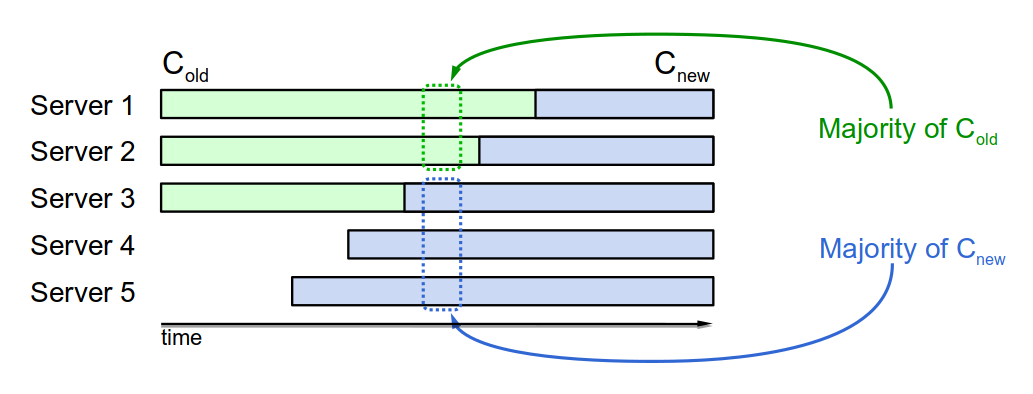
\includegraphics[scale=0.3]{raft-configuration-changes.png}
\end{frame}

\begin{frame}
    \frametitle{Joint Consensus}
    \begin{itemize}
        \item \textbf{Raft uses a 2-phase approach}
            \begin{itemize}
                \item Intermediate phase uses \alert{joint consensus}(need majority of both old and new configurations for elections, Commitment)
                \item Configuration changes is just a log entry; applied immediately on receipt(committed or not)
                \item Once joint consensus is committed, begin replicating log entry for final configuration
            \end{itemize}
    \end{itemize}
    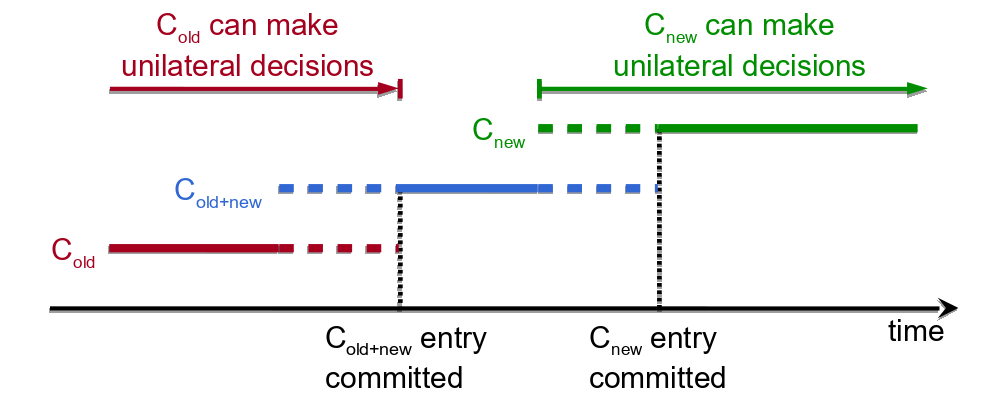
\includegraphics[scale=0.3]{raft-joint-consensus.png}
\end{frame}

\begin{frame}
    \frametitle{Joint Consensus, cont'd}
    \begin{itemize}
        \item \textbf{Additional details:}
            \begin{itemize}
                \item Any server from either configuration can serve as leader
                \item If current leader is not in $C_{new}$, must step down once $C_{new}$ is committed
            \end{itemize}
    \end{itemize}
    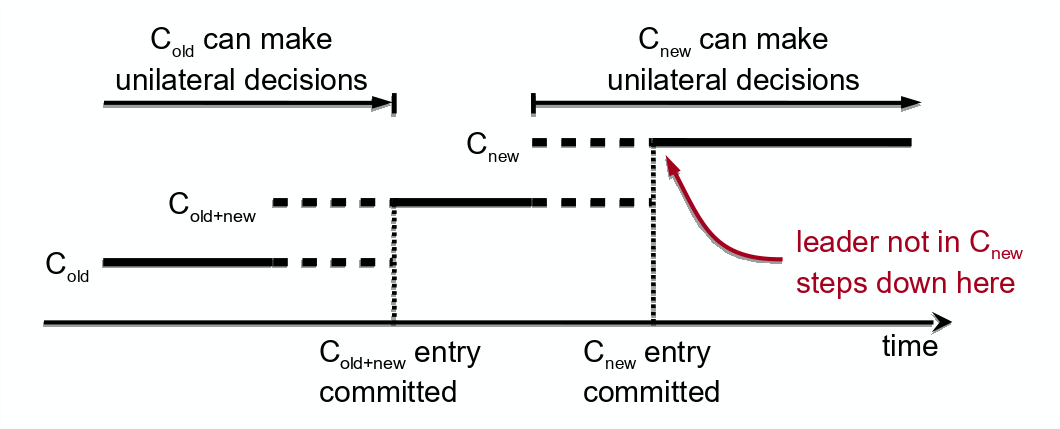
\includegraphics[scale=0.3]{raft-joint-consensus2.png}
\end{frame}




%\subsection{Paxos}

\begin{frame}
    \frametitle{Paxos Algorithm}
    \begin{itemize}
        \item Leslie Lamport, 1990
        \item Nearly synonymous with consensus
    \end{itemize}
    \begin{block}{The Chubby Author}
        \emph{There is only one consensus protocol, and that's Paxos, all other approaches are just broken versions of Paxos.} \\
    \end{block}
    \begin{block}{The Chubby Author}
        \emph{There are significant gaps between the description of the Paxos algorithm and the needs of a real-world system\ldots the final system will based on an unproven protocol.}
    \end{block}
\end{frame}

